% Created 2023-01-07 sáb 19:04
% Intended LaTeX compiler: pdflatex
\documentclass[aspectratio=169, usenames,svgnames,dvipsnames]{beamer}
\usepackage[utf8]{inputenc}
\usepackage[T1]{fontenc}
\usepackage{graphicx}
\usepackage{longtable}
\usepackage{wrapfig}
\usepackage{rotating}
\usepackage[normalem]{ulem}
\usepackage{amsmath}
\usepackage{amssymb}
\usepackage{capt-of}
\usepackage{hyperref}
\usepackage{color}
\usepackage{listings}
\usepackage{mathpazo}
\usepackage{gensymb}
\usepackage{amsmath}
\usepackage{diffcoeff}
\usepackage{steinmetz}
\usepackage{mathtools}
\bibliographystyle{plain}
\usepackage{siunitx}
\sisetup{output-decimal-marker={,}}
\DeclareSIUnit{\watthour}{Wh}
\hypersetup{colorlinks=true, linkcolor=Blue, urlcolor=Blue}
\renewcommand{\thefootnote}{\fnsymbol{footnote}}
\newcommand{\laplace}[1]{\mathbf{#1}(\mathbf{s})}
\newcommand{\slp}{\mathbf{s}}
\newcommand{\fasor}[1]{\mathbf{#1}(\omega)}
\newcommand{\atan}{\mathrm{atan}}
\parskip=5pt
\usetheme{Boadilla}
\usecolortheme{rose}
\usefonttheme{serif}
\author{Oscar Perpiñán Lamigueiro}
\date{}
\title{Elementos Activos}
\subtitle{Teoría de Circuitos II}
\setbeamercolor{alerted text}{fg=blue!50!black} \setbeamerfont{alerted text}{series=\bfseries}
\AtBeginSubsection[]{\begin{frame}[plain]\tableofcontents[currentsubsection,sectionstyle=show/shaded,subsectionstyle=show/shaded/hide]\end{frame}}
\AtBeginSection[]{\begin{frame}[plain]\tableofcontents[currentsection,hideallsubsections]\end{frame}}
\beamertemplatenavigationsymbolsempty
\setbeamertemplate{footline}[frame number]
\setbeamertemplate{itemize items}[triangle]
\setbeamertemplate{enumerate items}[circle]
\setbeamertemplate{section in toc}[circle]
\setbeamertemplate{subsection in toc}[circle]
\hypersetup{
 pdfauthor={Oscar Perpiñán Lamigueiro},
 pdftitle={Elementos Activos},
 pdfkeywords={},
 pdfsubject={},
 pdfcreator={Emacs 28.2 (Org mode 9.5.2)}, 
 pdflang={Spanish}}
\begin{document}

\maketitle

\section{Clasificación}
\label{sec:org0c08b84}
\begin{frame}[label={sec:org7e0905d}]{Tabla de Clasificación}
\begin{itemize}
\item Tensión o Corriente
\item Ideal o Real
\item Dependiente o Independiente
\end{itemize}
\end{frame}

\begin{frame}[label={sec:orga576bad}]{Generador Ideal}
\begin{columns}
\begin{column}{0.5\columnwidth}
\begin{center}
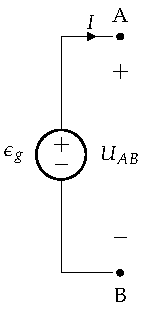
\includegraphics[height=0.5\textheight]{../figs/FuenteTensionIdealDC.pdf}
\end{center}
Un \alert{generador de tensión ideal} impone la tensión a la salida (\emph{la corriente depende del circuito}). Se caracteriza por su \alert{fuerza electromotriz} (voltios [V]).
\end{column}

\begin{column}{0.5\columnwidth}
\begin{center}
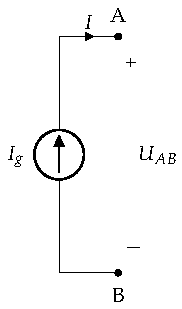
\includegraphics[height=0.5\textheight]{../figs/FuenteCorrienteIdeal.pdf}
\end{center}
Un \alert{generador de corriente ideal} impone la corriente a la salida (\emph{la tensión depende del circuito}). Se caracteriza por su corriente de generador.
\end{column}
\end{columns}
\end{frame}

\begin{frame}[label={sec:org09de0ec}]{Generador Real CC}
Los generadores reales tienen pérdidas que se modelan con una resistencia en \alert{serie} (generador de tensión) o en \alert{paralelo} (generador de corriente)

\begin{columns}
\begin{column}{0.5\columnwidth}
\begin{center}
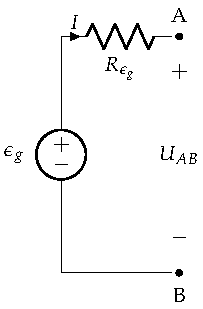
\includegraphics[height=0.7\textheight]{../figs/FuenteTensionRealDC.pdf}
\end{center}
\end{column}
\begin{column}{0.5\columnwidth}
\begin{center}
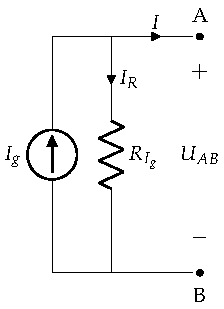
\includegraphics[height=0.7\textheight]{../figs/FuenteCorrienteRealDC.pdf}
\end{center}
\end{column}
\end{columns}
\end{frame}

\begin{frame}[label={sec:org9810986}]{Generador Real AC}
Los generadores reales tienen pérdidas que se modelan con una impedancia en \alert{serie} (generador de tensión) o en \alert{paralelo} (generador de corriente)

\begin{columns}
\begin{column}{0.5\columnwidth}
\begin{center}
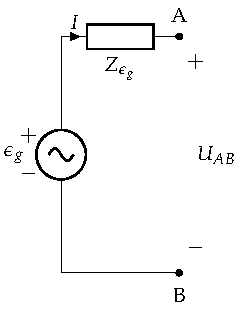
\includegraphics[height=0.5\textheight]{../figs/FuenteTensionReal.pdf}
\end{center}
\[
  \overline{U}_{AB} = \overline{\epsilon}_g - \overline{Z}_{\epsilon_g} \cdot \overline{I}
\]
\end{column}
\begin{column}{0.5\columnwidth}
\begin{center}
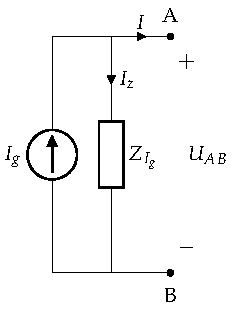
\includegraphics[height=0.5\textheight]{../figs/FuenteCorrienteReal.pdf}
\end{center}
\[
  \overline{I} = \overline{I}_g - \frac{\overline{U}_{AB}}{\overline{Z}_{I_g}}
\]
\end{column}
\end{columns}
\end{frame}


\begin{frame}[label={sec:orgf08f71f}]{Generadores Dependientes}
\begin{block}{Generadores de Tensión}
\begin{columns}
\begin{column}{0.5\columnwidth}
  \begin{center}
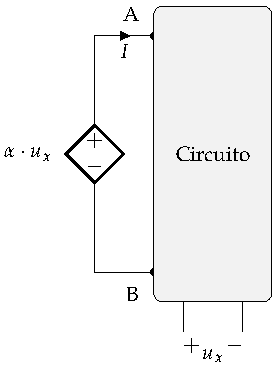
\includegraphics[height=0.7\textheight]{../figs/FuenteTensionDependienteTension.pdf}
\end{center}
\ldots{} de Tensión
\end{column}
\begin{column}{0.5\columnwidth}
  \begin{center}
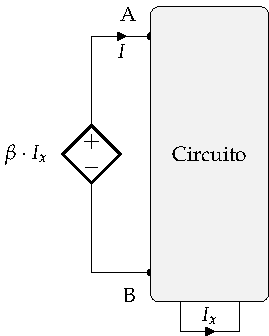
\includegraphics[height=0.7\textheight]{../figs/FuenteTensionDependienteCorriente.pdf}
\end{center}
\ldots{} de Corriente
\end{column}
\end{columns}
\end{block}
\begin{block}{Generadores de Corriente}
\begin{columns}
\begin{column}{0.5\columnwidth}
 \begin{center}
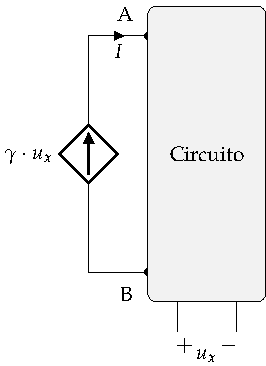
\includegraphics[height=0.7\textheight]{../figs/FuenteCorrienteDependienteTension.pdf}
\end{center}
\ldots{} de Tensión
\end{column}
\begin{column}{0.5\columnwidth}
 \begin{center}
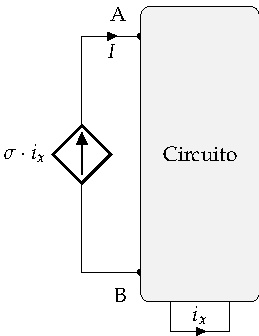
\includegraphics[height=0.7\textheight]{../figs/FuenteCorrienteDependienteCorriente.pdf}
\end{center}
\ldots{} de Corriente
\end{column}
\end{columns}
\end{block}
\end{frame}


\section{Generadores Independientes Reales}
\label{sec:org9487f2a}

\begin{frame}[label={sec:org14afe6b}]{Ecuación del generador CC}
\begin{columns}
\begin{column}{0.5\columnwidth}
\begin{center}
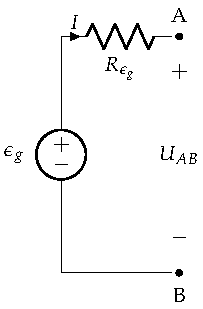
\includegraphics[height=0.5\textheight]{../figs/FuenteTensionRealDC.pdf}
\end{center}
\[
  U_{AB} = \epsilon_g - R_{\epsilon_g} \cdot I
\]
\end{column}
\begin{column}{0.5\columnwidth}
\begin{center}
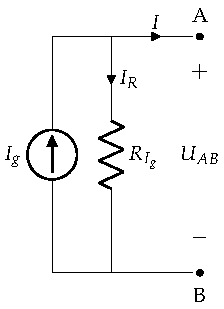
\includegraphics[height=0.5\textheight]{../figs/FuenteCorrienteRealDC.pdf}
\end{center}
\[
  I = I_g - \frac{U_{AB}}{R_{I_g}}
\]
\end{column}
\end{columns}
\end{frame}
\begin{frame}[label={sec:org4109791}]{Ecuación del generador AC}
\begin{columns}
\begin{column}{0.5\columnwidth}
\begin{center}
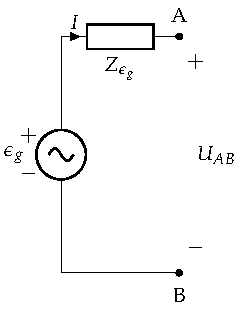
\includegraphics[height=0.5\textheight]{../figs/FuenteTensionReal.pdf}
\end{center}
\[
  \overline{U}_{AB} = \overline{\epsilon}_g - \overline{Z}_{\epsilon_g} \cdot \overline{I}
\]
\end{column}
\begin{column}{0.5\columnwidth}
\begin{center}
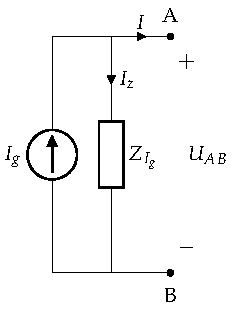
\includegraphics[height=0.5\textheight]{../figs/FuenteCorrienteReal.pdf}
\end{center}
\[
  \overline{I} = \overline{I}_g - \frac{\overline{U}_{AB}}{\overline{Z}_{I_g}}
\]
\end{column}
\end{columns}
\end{frame}

\begin{frame}[label={sec:org5808ff1}]{Diagramas Tensión - Corriente}
\begin{columns}
\begin{column}{0.5\columnwidth}
Fuente de tensión
\begin{center}
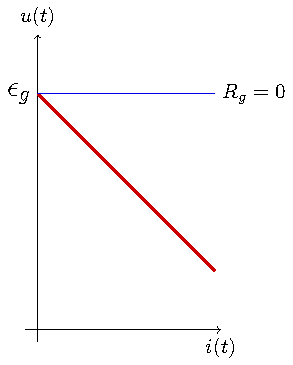
\includegraphics[height=0.5\textheight]{../figs/FuenteTension_DiagramaTensionCorriente.pdf}
\end{center}
\[
  u(t) = \epsilon_g - R_{\epsilon_g} \cdot i(t)
\]
\end{column}
\begin{column}{0.5\columnwidth}
Fuente de corriente
\begin{center}
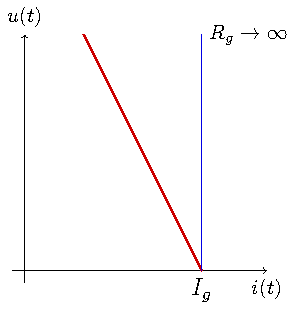
\includegraphics[height=0.5\textheight]{../figs/FuenteCorriente_DiagramaTensionCorriente.pdf}
\end{center}
\[
  u(t) = R_{I_g} \cdot I_g - R_{I_g} \cdot i(t)
\]
\end{column}
\end{columns}
\end{frame}
\begin{frame}[label={sec:orgb4cfaad}]{Potencia y rendimiento de una fuente}
\begin{columns}
\begin{column}{0.4\columnwidth}
\begin{center}
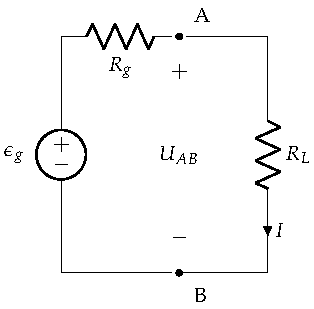
\includegraphics[height=0.55\textheight]{../figs/FuenteTensionRealConCarga.pdf}
\end{center}
\end{column}

\begin{column}{0.6\columnwidth}
\[
  \left.
    \begin{array}{c}
      I = \epsilon_g/(R_g + R_L)\\
      \\
      P_g = \epsilon_g \cdot I\\
      \\
      P_L = I^2 \cdot R_L
    \end{array} \right\}
  \rightarrow \left\{
    \begin{array}{c}
      P_g = \frac{\epsilon^2_g}{(R_g + R_L)}\\
      \\
      P_L = \frac{\epsilon^2_g \cdot R_L}{(R_g + R_L)^2}\\
      \\
      \eta = \frac{P_L}{P_g} = \frac{R_L}{R_g + R_L}
    \end{array}\right.
\]
\end{column}
\end{columns}
\end{frame}

\begin{frame}[label={sec:orgfd8f8a1}]{Potencia y rendimiento de una fuente}
\begin{columns}
\begin{column}{0.5\columnwidth}
\begin{itemize}
\item La potencia entregada por la fuente es máxima cuando \(R_L = R_g\).
\end{itemize}

\begin{equation*}
  P_L = \frac{\epsilon^2_{th}}{4 R_g}
\end{equation*}

\begin{itemize}
\item El rendimiento es una función creciente (\(\eta \to 1\) para \(R_L \gg R_g\)).
\end{itemize}
\end{column}

\begin{column}{0.5\columnwidth}
\begin{center}
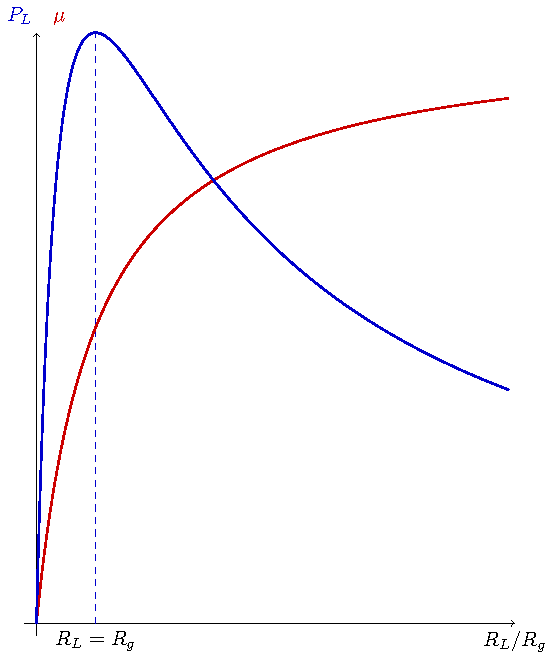
\includegraphics[height=0.85\textheight]{../figs/FuenteReal_PotenciaRendimiento.pdf}
\end{center}
\end{column}
\end{columns}
\end{frame}

\begin{frame}[label={sec:org76d924d}]{Potencia y rendimiento de una fuente}
\begin{columns}
\begin{column}{0.5\columnwidth}
\begin{itemize}
\item En la zona a la derecha del punto de máxima potencia (\(R_L > R_g\)), la función de potencia tiene una variación suave: los cambios en \(R_L\) tienen un impacto pequeño en \(P_L\).
\item Por ejemplo:
\begin{itemize}
\item Para \(R_L = R_g\) se obtiene \(\mu = 0'5\)
\item Para \(R_L = 2\cdot R_g\), se obtiene \(P_L = 0'89 \cdot P_{max}\) y \(\mu = 0'67\).
\item Para \(R_L = 3\cdot R_g\), se obtiene \(P_L = 0'75 \cdot P_{max}\) y \(\mu = 0'75\).
\end{itemize}
\end{itemize}
\end{column}
\begin{column}{0.5\columnwidth}
\begin{center}
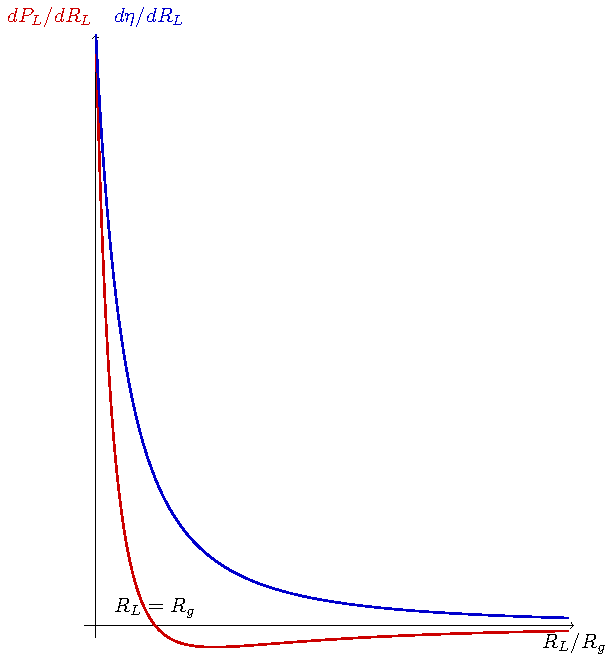
\includegraphics[height=0.85\textheight]{../figs/FuenteReal_DifPotencia.pdf}
\end{center}
\end{column}
\end{columns}
\end{frame}


\section{Transformación y Asociación}
\label{sec:org7e62417}
\begin{frame}[label={sec:orgc06db2f}]{Equivalencia de fuentes}
Sólo es posible establecer equivalencia entre \alert{fuentes reales}.
\begin{columns}
\begin{column}{0.33\columnwidth}
\begin{center}
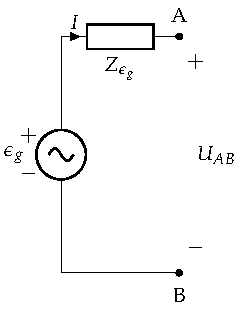
\includegraphics[height=0.5\textheight]{../figs/FuenteTensionReal.pdf}
\end{center}
\[
  \overline{U}_{AB} = \overline{\epsilon}_g - \overline{Z}_{\epsilon_g} \cdot \overline{I}
\]
\end{column}
\begin{column}{0.33\columnwidth}
\begin{align*}
  \overline{Z}_g &= \overline{Z}_{\epsilon_g} = \overline{Z}_{I_g}\\
  \overline{\epsilon}_g &= \overline{Z}_g \cdot \overline{I}_g\\
  \overline{I}_g &= \frac{\overline{\epsilon}_g}{\overline{Z}_g}
\end{align*}
\end{column}
\begin{column}{0.33\columnwidth}
\begin{center}
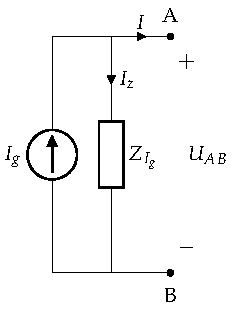
\includegraphics[height=0.5\textheight]{../figs/FuenteCorrienteReal.pdf}
\end{center}
\[
  \overline{I} = \overline{I}_g - \frac{\overline{U}_{AB}}{\overline{Z}_{I_g}}
\]
\end{column}
\end{columns}
\end{frame}


\begin{frame}[label={sec:org9799bf0}]{Conexión en serie de generadores}
\begin{block}{Generadores de Tensión}
\begin{itemize}
\item Pueden conectarse en serie sin restricción.

\begin{align*}
  \epsilon_T &= \sum_{i = 1}^N \epsilon_i\\
  R_{gT} &= \sum_{i = 1}^N R_{gi}\\ 
\end{align*}
\end{itemize}
\end{block}

\begin{block}{Generadores de Corriente}
\begin{itemize}
\item Ideal: todas las fuentes deben ser idénticas (valor y sentido).
\item Real:  sin restricción, transformación de fuentes para fuente equivalente.
\end{itemize}
\end{block}
\end{frame}


\begin{frame}[label={sec:org942c707}]{Conexión en paralelo de generadores}
\begin{block}{Generadores de Tensión}
\begin{itemize}
\item Ideal: todas las fuentes deben ser idénticas (valor y polaridad).
\item Real:  sin restricción, transformación de fuentes para fuente equivalente.
\end{itemize}
\end{block}


\begin{block}{Generadores de Corriente}
\begin{itemize}
\item Pueden conectarse en paralelo sin restricción.

\begin{align*}
  I_{gT} &= \sum_{i = 1}^N I_{gi}\\
  G_{gT} &= \sum_{i = 1}^N G_{gi}\\ 
\end{align*}
\end{itemize}
\end{block}
\end{frame}




\begin{frame}[label={sec:orgb21fa58}]{Fuentes dominantes}
\end{frame}

\begin{frame}[label={sec:orgbfba0f9}]{Modificación de la geometría de un circuito}
Apartado 6 (p. 185) Pastor
\end{frame}
\end{document}